% Copyright (C) 2017 by SIB Swiss Institute of Bioinformatics, Julien Dorier and Dimos Goundaroulis.
% 
% This file is part of project Knoto-ID.
% 
% Knoto-ID is free software: you can redistribute it and/or modify
% it under the terms of the GNU General Public License as published by
% the Free Software Foundation, either version 2 of the License, or
% (at your option) any later version.
% 
% Knoto-ID is distributed in the hope that it will be useful,
% but WITHOUT ANY WARRANTY; without even the implied warranty of
% MERCHANTABILITY or FITNESS FOR A PARTICULAR PURPOSE.  See the
% GNU General Public License for more details.
% 
% You should have received a copy of the GNU General Public License
% along with Knoto-ID.  If not, see <http://www.gnu.org/licenses/>.

\section{\label{sec:theory}Theory}
\subsection{\label{sec:theory:knots}Knots}
A knot is a smooth embedding of a circle into $\mathbb{R}^3$, considered up to continuous deformations. To be more precise, a knot is a closed curve in 3-dimensional Euclidean space that does not intersect itself anywhere and can be continuously deformed as if it was made of rubber\cite{Adams}.  Knots are usually studied through their diagrams, which are abstract and schematized pictures of a knot composed of curves in the plane that cross transversely in 4-fold vertices. Each vertex is equipped with extra structure in the form of a deleted segment that indicates the under crossing line and they are called {\it crossings} of the knot. With this information, one is always able to reconstruct the knot in 3-space (see Fig.~\ref{fig:knotdiag}).
\begin{figure}[h]
\centering
\subfloat[]{
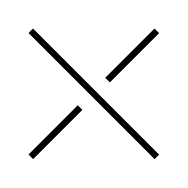
\begin{tikzpicture}[scale=.8]
\draw [line width=0.8mm]  (-1,-1)-- (-0.22,-0.22);
\draw  [line width=0.8mm ](-1,1)--(0,0);
\draw  [line width=0.8mm] (0.22,0.22) -- (1,1);
\draw [line width=0.8mm]   (0,0) -- +(1,-1);
\end{tikzpicture}}\hspace{3cm}
\subfloat[]{\includegraphics[scale=.13]{figure1}}
\caption{A crossing (a) and a knot diagram (b).}\label{fig:knotdiag}
\end{figure}


Two knots are equivalent, that is they can be deformed to one another, if and only if their diagrams can be transformed to one another by a finite sequence of three elementary diagram moves called the Reidemeister moves (see Fig.~\ref{fig:rmoves}) along with planar isotopy. Planar isotopy is a motion of the diagram in the plane that preserves the underlying structure. These tools work efficiently well for distinguishing knots with small number of crossings, however, for knots with higher number of crossings (see Fig.~\ref{fig:unknot}) more sophisticated tools are required.
\begin{figure}[h]
\centering
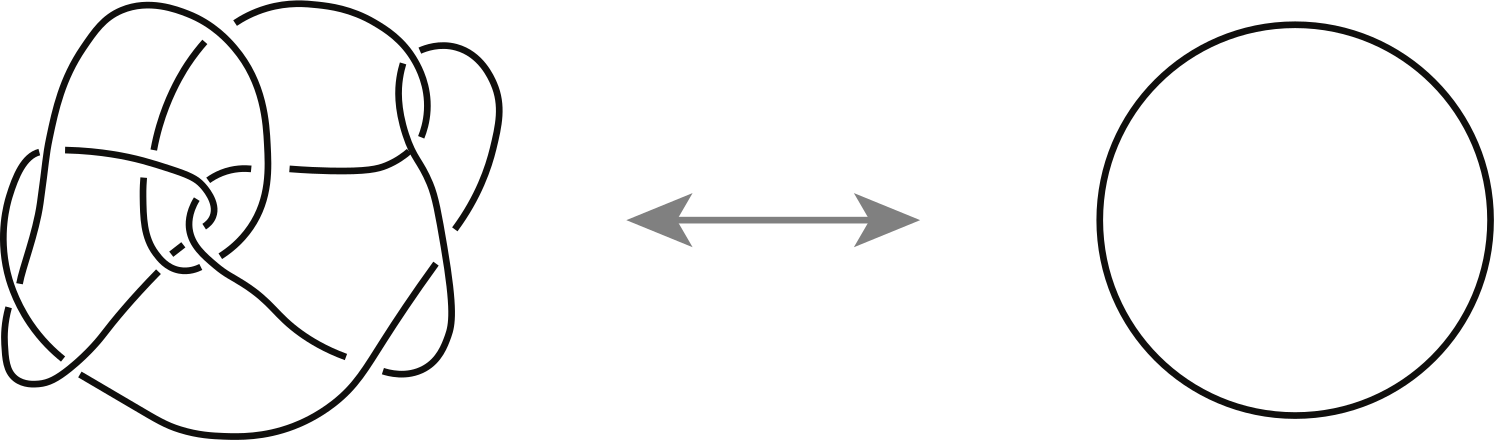
\includegraphics[scale=.3]{figure2}
\caption{Louis Kauffman's unknot. This rather complicated knot is actually equivalent to the trivial knot.}\label{fig:unknot}
\end{figure}

 Such tools are the so-called knot invariants and are functions defined on the set of all knots and links that assign the same value to equivalent knots or links. In this work we focus on the classical Jones polynomial for knots \cite{jones} and the various extensions of the Kauffman bracket polynomial \cite{kauffman1988} to the case of knotoids\cite{turaev,guka,gound2,goundaroulis2019}.

\begin{figure}[h]
\centering
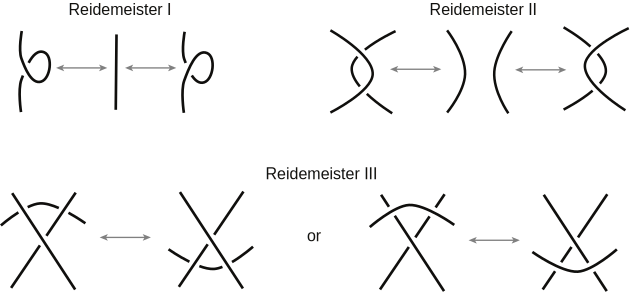
\includegraphics[scale=.93]{figure3}
\caption{The three Reidemeister moves.}\label{fig:rmoves}
\end{figure}


\subsection{\label{sec:theory:knotoids}Knotoids}
Consider that we started drawing a knot diagram and at some point in this process we decided to leave the diagram open, i.e. not to connect the end points. The question now is if this allows the definition of open knot diagrams. It is not difficult to see that if we apply planar isotopy and the Reidemeister moves as described above to such a diagram, eventually we will always manage to unknot it. However, if we require the Reidemeister moves to be applied only at local neighbourhoods of the diagram that don't involve the endpoints we are getting closer to the notion of open knotting. Additionally, if we forbid the endpoints to slide over or under the rest of the diagram (see Fig.~\ref{fig:forbidden}), then we have achieved our goal. 

\begin{figure}[h]
\centering
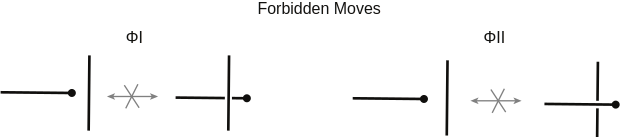
\includegraphics[scale=1]{figure4}
\caption{The two forbidden moves.}\label{fig:forbidden}
\end{figure}

What we have just described is a {\it knotoid diagram}. Knotoid diagrams generalize the notion of a 1-1 tangle (or a long knot) since they allow the endpoints to be in different regions of the diagram, and thus they provide a rigorous definition for open knots. Their equivalence classes under the forbidden moves as well as the Reidemeister moves away from the endpoints  are called {\it knotoids} (see Fig.~\ref{fig:knotoid}). Knotoids were first introduced by V. Turaev in\cite{turaev} and have been studied further by L. Kauffman and N. G\"ug\"umc\"u in\cite{guka}.  Formally, a knotoid is defined as the generic  immersion  of  the  closed unit interval  in  the  interior  of the surface whose  only  singularities are  transversal  double  points  endowed  with  over/undercrossing  data. In analogy to the case of knots, the double points of the knotoid diagram are also called crossings.   The  images  of  0 and  1  under  this  immersion  are  called  the {\it tail} and  the {\it head} of the knotoid diagram,  respectively, they are  distinct  from  each other  and from  the  double  points.  Every knotoid diagram comes with an orientation the goes from the tail to the head\cite{turaev}.  Knotoids that have both ends in the same region of the diagram are called {\it knot-type} knotoids while knotoids that have their end points in different regions of the diagram are called {\it proper} knotoids.

\begin{figure}[h]
\centering
\includegraphics[scale=.35]{figure5}
\caption{Examples of knotoids. The diagram (c) corresponds to a knot-type knotoid while (a), (b) and (d) to proper knotoids.}\label{fig:knotoid}
\end{figure}

Knotoids are defined on an oriented surface but they are usually studied on the surface of the 2-sphere $S^2$ but their definition can also be extended to the plane $\mathbb{R}^2$. We shall call this class of knotoids {\it planar}. There are pairs non-isotopic planar knotoids that become isotopic once we consider them as knotoids on $S^2$. For example, in Figure~\ref{fig:knotoid}, diagrams (a) and (b) are not equivalent as planar knotoids but they become equivalent once they are considered in $S^2$. This is because on the sphere one has the freedom to move arcs using isotopy towards/over the poles and around the sphere in order to simplify the diagram, something that is not possible while working on the plane.


One can recover a knot diagram from a knotoid diagram $k$ by embedding an arc $\alpha$ that passes everywhere under $k$ and connect the endpoints of $k$ to $\alpha$. The arc is called a {\it shortcut} for $k$ and the way of closure is called the {\it underpass} closure  (See Figure~\ref{fig:closure}). The shortcut is unique for every knotoid diagram, up to isotopy. In an analogous way one can define the {\it overpass closure}\cite{turaev, guka}. On the other hand, every knot may be presented by a knotoid diagram by cutting out an underpassing arc\cite{turaev}.


\begin{figure}[h]
\centering
\includegraphics[scale=.35]{figure6}
\caption{Knotoids to knots using the underpass closure. The embedded arc $\alpha$ is shown in red.}\label{fig:closure}
\end{figure}





\subsection{\label{sec:theory:knotoidsandcurves}Knotoids and curves in space}

Consider an embedded open curve in space. We would like to know if it is entangled or not. One may suggest to project the curve on a plane and study its projection as a knotoid diagram and they would be partially right. However, how can we be sure that by accidentally perturbing a bit the curve we don't mess with its topology? In order to avoid situations like this we first introduce two infinite lines that pass through the endpoints of the curve. In this way all manipulations of the curve in space with respect to these two lines preserve the topology of the curve\cite{guka}. Finally, the curve is projected on  an orientable surface (e.g. a sphere, a plane, etc.), and thus a knotoid diagram is obtained. 

Note now that different choices of projection planes will possibly lead to different knotoid diagrams. For this reason, in order to study the topology of an embedded open curve we work as follows. We assume that the curve lies inside a large enough sphere (a radius of twice the length of the curve will do fine for most of the cases). Each point of the sphere corresponds to a vector that points towards an orientable surface that lies outside of the sphere (see Figure~\ref{fig:project}). For each choice of the projection surface we introduce the infinite parallel lines and we take the projection of the curve together with the information of over/under crossing arc at each double point. The knotoid type is then evaluated using an invariant for knotoids. Thus, the entanglement of the embedded open curve is a probability distribution that we can approximate by sampling the sphere\cite{gound}.
\begin{figure}[h]
\centering
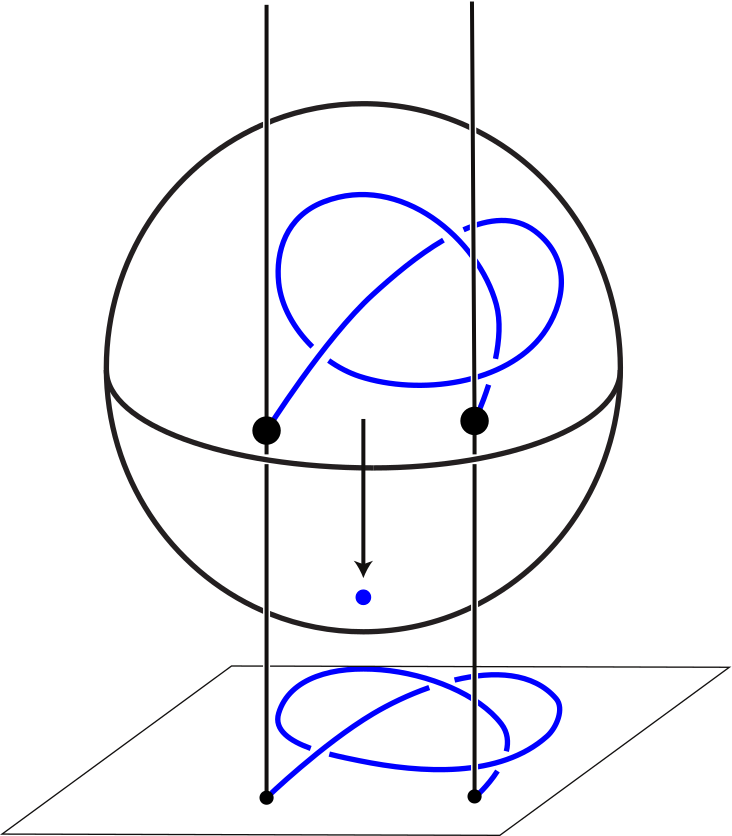
\includegraphics[scale=.3]{figure7}
\caption{ The curve is placed inside a large sphere. The blue dot indicates a vector that points towards an oriented surface of projection (plane or sphere). The two infinite parallel lines are introduced and the curve is projected on the chosen oriented surface.}\label{fig:project}
\end{figure}


The equivalent of the over/underpassing closure for the case of embedded open curves is most probably the uniform (or stochastic) closure technique\cite{mansfield1994, sulkowska2012, lua2006,millett2004, jamroz2014}.
Here the curve is placed again inside a large ball, only this time each point of the sphere corresponds to a closure direction. The closure is achieved by extending two parallel rays, each originating from one of the endpoints of the curve, towards that the chosen closure direction and they are connected outside of the sphere (see Figure~\ref{fig:closure}).
This method is, as hinted by its name, also probabilistic and so the knot-type of the core is a probability distribution of all knot-types obtained by closing over all possible directions that are defined by the points of the sphere.
There is however the option to close the open curve using an arc that directly connects the endpoints\cite{taylor2000,virnau2006} (direct closure method). This method is computationally faster but it may interfere with the topology of the chain by introducing or removing crossings. In contrast to the direct closure technique, the stochastic closure provides more detailed overview but it is computationally more demanding as one is required to sample a probability distribution in order to understand the topology of the studied object.
\begin{figure}[h]
\centering
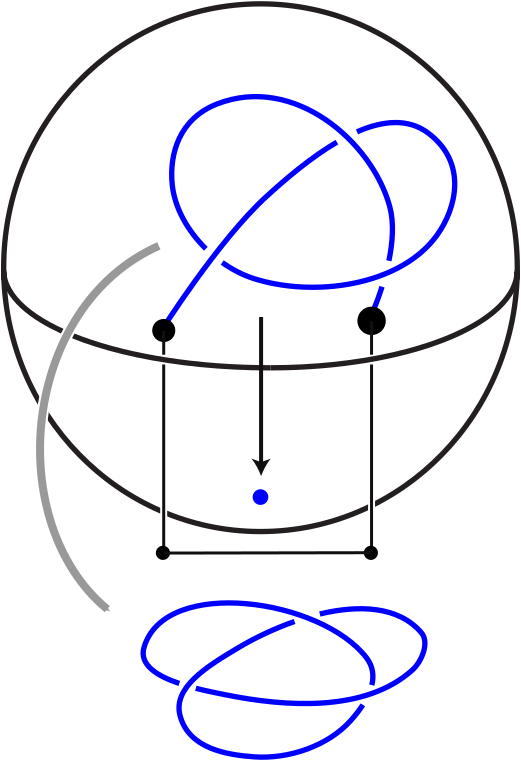
\includegraphics[scale=.3]{figure8}
\caption{The uniform (or stochastic) closure technique. Two parallel rays are extended towards the closure direction indicated by the blue point and they are connected outside of the sphere. The resulting knot may be evaluated using a knot invariant.}\label{fig:stochastic}
\end{figure}

\subsection{\label{sec:theory:jones}Computing polynomial invariants}
In this section we will present the Kauffman bracket\cite{kauffman1988} and how it gives rise to the classical Jones polynomial for knots\cite{jones}, the Jones polynomial for knotoids\cite{turaev,guka} and the Turaev loop bracket polynomial for planar knotoids\cite{turaev}. Moreover, we present how we can obtain the arrow polynomial \cite{dye2009,guka} from the oriented extension of the Kauffman bracket. Finally, we give the planar extension of the arrow polynomial, the loop arrow polynomial \cite{gound2, goundaroulis2019}

\subsubsection{\label{sec:theory:jones:classicaljones}Classical Jones polynomial for knots}
Consider  a knot $K$ and observe that a each crossing \raisebox{-.1cm}{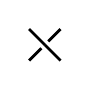
\begin{tikzpicture}[scale=.2]
\draw [line width=0.35mm]  (-1,-1)-- (-0.22,-0.22);
\draw  [line width=0.35mm ](-1,1)--(0,0);
\draw  [line width=0.35mm] (0.22,0.22) -- (1,1);
\draw [line width=0.35mm]   (0,0) -- +(1,-1);
\end{tikzpicture}} of $K$ can be smoothed in two different ways. The first way is to smooth it horizontally \raisebox{-.07cm}{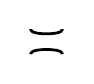
\begin{tikzpicture}[scale=.2]
\draw [line width=0.35mm] plot [smooth, tension=2] coordinates { (-1,.8) (0, 0.5) (1,.8)};
\draw [ line width=0.35mm] plot [smooth, tension=2] coordinates { (-1,-.8) (0, -0.5) (1,-.8)};
\end{tikzpicture}} and the second is to smooth it vertically  \raisebox{-.1cm}{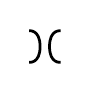
\begin{tikzpicture}[scale=.2]
 \draw [ line width=0.35mm] plot [smooth, tension=2] coordinates { (-1,-1) (-0.3, 0) (-1,1)};
 \draw [ line width=0.35mm] plot [smooth, tension=2] coordinates { (1,-1) (0.3, 0) (1,1)};
 \end{tikzpicture}}. If $K$ has $n$ crossings then  there are $2^n$ possible smoothings of $K$. With these in mind we define the Kauffman bracket as the 1-variable polynomial $\langle K \rangle \in \mathbb{Z}[A,A^{-1}]$ that satisfies the following axioms:


\begin{eqnarray}
&&\langle \raisebox{-.1cm}{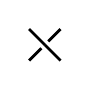
\begin{tikzpicture}[scale=.2]
\draw [line width=0.35mm]  (-1,-1)-- (-0.22,-0.22);
\draw  [line width=0.35mm ](-1,1)--(0,0);
\draw  [line width=0.35mm] (0.22,0.22) -- (1,1);
\draw [line width=0.35mm]   (0,0) -- +(1,-1);
\end{tikzpicture}}\, \rangle =A \langle \, \raisebox{-.07cm}{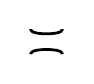
\begin{tikzpicture}[scale=.2]
\draw [line width=0.35mm] plot [smooth, tension=2] coordinates { (-1,.8) (0, 0.5) (1,.8)};
\draw [ line width=0.35mm] plot [smooth, tension=2] coordinates { (-1,-.8) (0, -0.5) (1,-.8)};
\end{tikzpicture}}\, \rangle   + A^{-1} \,\langle\, \raisebox{-.1cm}{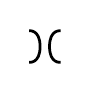
\begin{tikzpicture}[scale=.2]
 \draw [ line width=0.35mm] plot [smooth, tension=2] coordinates { (-1,-1) (-0.3, 0) (-1,1)};
 \draw [ line width=0.35mm] plot [smooth, tension=2] coordinates { (1,-1) (0.3, 0) (1,1)};
 \end{tikzpicture}}\, \rangle \label{regbracket1} \\
&&\langle K \sqcup \bigcirc \rangle = \left (-A^2 - A^{-2}\right ) \langle K \rangle \\
&&  \langle \, \bigcirc \, \rangle  = 1 
\end{eqnarray}

The first axiom gives the smoothing rule on a local region of the knot diagram. This means that  all three diagrams in \ref{regbracket1} are identical everywhere except in the region that is shown inside the brackets. The second axiom tells us that a disjoint circle from the rest of the diagram multiplies the diagram by $(-A^2 - A^{-2})$. The last axiom is the basis of the inductive process. Note that the Kauffman bracket polynomial is invariant under the second and the third Reidemeister moves but not under the first Reidemeister move. In order to establish invariance under the first move,  we choose an orientation for the knot diagram, i.e. we assign a direction indicated by arrows on its arcs. The crossings in an oriented diagram are given signs of $\pm 1$ (see Fig.~\ref{crossings})

\begin{figure}[h]
\centering
\subfloat[]{
 \raisebox{-.1cm}{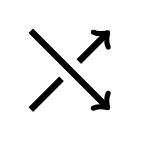
\begin{tikzpicture}[scale=.5]
\draw [line width=0.8mm]  (-1,-1)-- (-0.22,-0.22);
\draw  [line width=0.8mm](-1,1)--(0,0);
\draw  [line width=0.8mm] (0.22,0.22) -- (1,1)[->];
\draw [line width=0.8mm]   (0,0) -- +(1,-1)[->];
\end{tikzpicture}}}   \hspace{3cm}
\subfloat[]{ \raisebox{-.1cm}{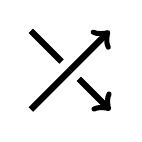
\begin{tikzpicture}[scale=.5]
\draw  [line width=0.8mm] (-1,-1)-- (0,0) ;
\draw [line width=0.8mm] (-1,1)--(-0.22,0.22);
\draw [line width=0.8mm] (0,0) -- (1,1)[->];
\draw [line width=0.8mm]   (0.22,-0.22) -- +(.8,-.8)[->];
\end{tikzpicture}}}
\caption{A positive crossing with sign +1 (a) and a negative crossing with sign -1 (b).}\label{crossings}
\end{figure}

The sum of signs of all crossings of a knot diagram $K$ is called {\it the writhe} of $K$, ${\rm wr}(K)$, and it will allow us to make the Kauffman bracket invariant under the first Reidemeister move. Indeed, by considering the following normalization of the Kauffman bracket,  we have achieved our goal.
\begin{equation}\label{jones}
f_K(A) = (-A^3)^{- {\rm wr}(K)} \langle K \rangle,
\end{equation}
where $\langle K \rangle$ is the Kauffman bracket polynomial of $K$. It turns out the $f_K(A)$ coincides with the classical Jones polynomial.

\subsubsection{\label{sec:theory:jones:jonesknotoids}Jones polynomial for knotoids}
One may extend the definition of the Kauffman bracket and, in turn of the classical Jones Polynomial, to the case of knotoids. The rules are more or less the same, with some minor tweaks depending on whether we want compute the invariant for a knotoid in $S^2$ or a planar knotoid. Knotoids are open ended diagrams and therefore when one smoothes all crossings of the diagram, in the end they will always end up with a number of disjoint circles and a single long segment. We choose the long segment to be the basis of the inductive procedure and so the axioms for a knotoid diagram $k$ become as follows:
\begin{eqnarray}
&&\langle \raisebox{-.1cm}{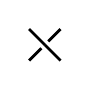
\begin{tikzpicture}[scale=.2]
\draw [line width=0.35mm]  (-1,-1)-- (-0.22,-0.22);
\draw  [line width=0.35mm ](-1,1)--(0,0);
\draw  [line width=0.35mm] (0.22,0.22) -- (1,1);
\draw [line width=0.35mm]   (0,0) -- +(1,-1);
\end{tikzpicture}}\, \rangle =A \langle \, \raisebox{-.07cm}{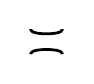
\begin{tikzpicture}[scale=.2]
\draw [line width=0.35mm] plot [smooth, tension=2] coordinates { (-1,.8) (0, 0.5) (1,.8)};
\draw [ line width=0.35mm] plot [smooth, tension=2] coordinates { (-1,-.8) (0, -0.5) (1,-.8)};
\end{tikzpicture}}\, \rangle   + A^{-1} \,\langle\, \raisebox{-.1cm}{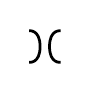
\begin{tikzpicture}[scale=.2]
 \draw [ line width=0.35mm] plot [smooth, tension=2] coordinates { (-1,-1) (-0.3, 0) (-1,1)};
 \draw [ line width=0.35mm] plot [smooth, tension=2] coordinates { (1,-1) (0.3, 0) (1,1)};
 \end{tikzpicture}}\, \rangle  \\
&&\langle k \sqcup \bigcirc \rangle = \left (-A^2 - A^{-2}\right ) \langle k \rangle\\
&&  \langle \, \raisebox{.07cm}{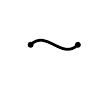
\begin{tikzpicture}[scale=.1, baseline]
\draw[line width=0.35mm] 
  (1,0) 
    .. controls (3,2) and (5,-2) .. 
  (7,0);  
\draw[black,fill=black] (1,0) circle (2ex);
\draw[black,fill=black] (7,0) circle (2ex);
\end{tikzpicture}}\, \rangle  = 1 \label{regbracket3}
\end{eqnarray}

The invariance unde the first Reidemeister move is taken care by the same normalization as with the case of knots.
\begin{equation}\label{jonesknotoids}
J_k(A) = (-A^3)^{- {\rm wr}(k)} \langle k \rangle,
\end{equation}

where $\langle k \rangle$ is the Kauffman bracket polynomial of a knotoid diagram $k$ and ${\rm wr}(k)$ is the writhe of $k$. Equation~\ref{jonesknotoids} is the extension of the classical Jones for the case of knotoids in $S^2$.
\subsubsection{\label{sec:theory:jones:jonesknotoids}Turaev loop bracket polynomial for planar knotoids}
The case of planar knotoids requires some more explanation. As mentioned above when one smoothes all crossings of a knotoid diagram, they will end up with a number of disjoint circles and one long segment. When we work on the surface of a 2-sphere, it doesn't matter whether the long segment rests inside a circle or not because, even if it does, we can always take it out by moving an arc of the circle around the surface of the sphere. If we work with planar knotoids, we cannot do this and so we want to keep track of this information, i.e. if the long segments is inside a circle or not. For this reason, we add an extra variable to the Kauffman bracket polynomial that counts the number of circles that enclose the long segment in each possible smoothing of the knotoid diagram $k$.

\begin{eqnarray}
&&\langle \raisebox{-.1cm}{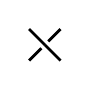
\begin{tikzpicture}[scale=.2]
\draw [line width=0.35mm]  (-1,-1)-- (-0.22,-0.22);
\draw  [line width=0.35mm ](-1,1)--(0,0);
\draw  [line width=0.35mm] (0.22,0.22) -- (1,1);
\draw [line width=0.35mm]   (0,0) -- +(1,-1);
\end{tikzpicture}}\, \rangle_{\circ}=A \langle \, \raisebox{-.07cm}{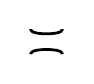
\begin{tikzpicture}[scale=.2]
\draw [line width=0.35mm] plot [smooth, tension=2] coordinates { (-1,.8) (0, 0.5) (1,.8)};
\draw [ line width=0.35mm] plot [smooth, tension=2] coordinates { (-1,-.8) (0, -0.5) (1,-.8)};
\end{tikzpicture}}\, \rangle_{\circ}   + A^{-1} \,\langle\, \raisebox{-.1cm}{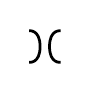
\begin{tikzpicture}[scale=.2]
 \draw [ line width=0.35mm] plot [smooth, tension=2] coordinates { (-1,-1) (-0.3, 0) (-1,1)};
 \draw [ line width=0.35mm] plot [smooth, tension=2] coordinates { (1,-1) (0.3, 0) (1,1)};
 \end{tikzpicture}}\, \rangle_{\circ} \label{regbracket1} \\
&&\langle K \sqcup \bigcirc \rangle_{\circ} = \left (-A^2 - A^{-2}\right ) \langle K \rangle_{\circ} \label{regbracket2}\\
&&\langle \ 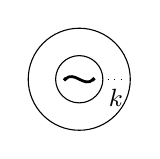
\begin{tikzpicture}[scale=.06,baseline]
        \draw (4,0) circle (5);
        \draw (4,0) circle (10.8);
         \draw[line width=0.35mm] 
  (1,0) 
    .. controls (3,2) and (5,-2) .. 
  (7,0);  
\draw[black,fill=black] (1,0) circle (2ex);
\draw[black,fill=black] (7,0) circle (2ex);
\draw[dotted] (0:10) -- node[below] {{\small $k$}} (0:13.5);
           \end{tikzpicture}
           \
            \rangle_{\circ} = v^k \label{regbracket3}\\
&&  \langle \, \raisebox{.07cm}{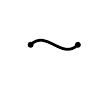
\begin{tikzpicture}[scale=.1, baseline]
\draw[line width=0.35mm] 
  (1,0) 
    .. controls (3,2) and (5,-2) .. 
  (7,0);  
\draw[black,fill=black] (1,0) circle (2ex);
\draw[black,fill=black] (7,0) circle (2ex);
\end{tikzpicture}}\, \rangle_{\circ}  = 1 \label{regbracket4}
\end{eqnarray}

This version of the bracket is a Laurent polynomial in $\mathbb{Z}[A,A^{-1},v]$. The invariance under the first Reidemeister move is given again by the same normalization:
\begin{equation}\label{loopbracket}
\widehat{J}_k(A, v) = (-A^3)^{- {\rm wr}(k)} \langle k \rangle_{\circ},
\end{equation}
where $ \langle k \rangle_{\circ}$ is an evaluation of the diagram $k$ using the rules described above.  The Turaev loop bracket polynomial is  defined by the Equation~\ref{loopbracket} and is an extension of the classical Jones polynomial to the case of planar knotoids.

\subsubsection{The arrow polynomial}

The arrow polynomial is based on the oriented expansion of the bracket polynomial and it was initially  defined in \cite{dye2009} as an invariant for virtual knots. It is a Laurent polynomial in the ring $\mathbb{Z}[A^{\pm1}, L_1, L_2, \ldots ]$, where the $L_i$ are an infinite set of independent commuting variables that also commute with the
Laurent polynomial variable $A$. The extension to classical knotoids in $S^2$ and virtual knotoids appeared in \cite{guka}. The skein relation in this case involves  smoothings with matching or conflicting orientations (see Eqs.~\ref{eq:arrow1} - \ref{eq:arrow5}).
\begin{eqnarray}
&&\raisebox{-0.5\height}{\includegraphics{arrow_skeinrelations_1}} \label{eq:arrow1}\\
&&\raisebox{-0.5\height}{\includegraphics{arrow_skeinrelations_2}}\label{eq:arrow2}\\
&&\raisebox{-0.5\height}{\includegraphics{arrow_skeinrelations_3}}\label{eq:arrow3}\\
&&\raisebox{-0.5\height}{\includegraphics{arrow_skeinrelations_4}}\label{eq:arrow4}\\
&&\raisebox{-0.5\height}{\includegraphics{arrow_skeinrelations_5}}\label{eq:arrow5}
\end{eqnarray}


 Note that each smoothing with a conflicting orientation results in a pair of cusps and, therefore, the set of axioms  for the recursive definition of the arrow polynomial \`{a} la bracket polynomial has to include rules that take into account these additional combinatorial structures. Each state includes a number of circular components and a long segment component, all of which may contain a number of consecutive cusps. A cancellation rule allows the simplification of two consecutive cusps into a straight arc, if the acute angles of both cusps are in the same local region of the diagram (see Fig.~\ref{fig:cancel}). The cancellation rule is not applicable to cases where the acute angles of two consecutive cusps are in different local regions of the diagram. 
 The arrow polynomial assigns a new variable to each long segment of a state with a number of surviving cusps. In particular, two consecutive surviving cusps form a zigzag and a long segment with $2i$ surviving cusps is evaluated at $m_i$. The skein relation together with the axioms discussed above define recursively the arrow polynomial. The arrow polynomial becomes an ambient isotopy invariant under the following normalization:

\begin{equation}\label{eq:arrow}
\mathcal{A}(k) = \left( - A^3 \right )^{-{\rm wr}(k)} \left [ k  \right ],
\end{equation}
where $ \left [ k  \right ]$ is an evaluation of the diagram $k$ using the rules described above.
 \begin{figure}[h] 
\centering
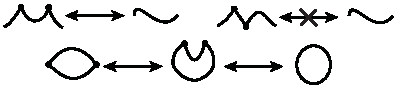
\includegraphics{figure_9}
\caption{\footnotesize The allowed and the forbidden cancellation rules.}\label{fig:cancel}
\end{figure}

\subsubsection{The loop arrow polynomial}

In analogy to the Turaev loop bracket, the loop arrow polynomial is the planar version of the arrow polynomial and it was mentioned first in \cite{gound2}. It is also a Laurent polynomial and it is lies in the ring 
\[
\mathbb{Z}[A^{\pm1}, v, m_1, m_2, \ldots, w_1, w_2, \ldots, p_1, p_2 \ldots, q_1, q_2, \ldots ],
\] where the $m_i$, $w_j$, $p_k$, $q_\ell$ are infinite sets of independent commuting variables that also commute with the
Laurent polynomial variables $A$ and $v$.  The loop arrow distinguishes two different types of zigzags (compare the zigzags in Eq.~\ref{eq:arrow4} to those in Eqs.~\ref{eq:loop_arrow1} and \ref{eq:loop_arrow2}) and it assigns one of the variables  $m_k$ or $w_i$, depending on the type of zigzag. Furthermore, much like the Turaev loop bracket, the loop arrow polynomial assigns different variables to circular components that enclose the long segment with or without any of the two types of zigzags. The loop arrow polynomial is defined by the rules of the arrow polynomial plus the additional rules in in Eqs.~\ref{eq:loop_arrow1}-\ref{eq:loop_arrow5}. 
\begin{eqnarray}
&&\raisebox{-0.5\height}{\includegraphics{loop_arrow_skeinrelations_1}}\label{eq:loop_arrow1}\\
&&\raisebox{-0.5\height}{\includegraphics{loop_arrow_skeinrelations_2}}\label{eq:loop_arrow2}\\
&&\raisebox{-0.5\height}{\includegraphics{loop_arrow_skeinrelations_3}}\label{eq:loop_arrow3}\\
&&\raisebox{-0.5\height}{\includegraphics{loop_arrow_skeinrelations_4}}\label{eq:loop_arrow4}\\
&&\raisebox{-0.5\height}{\includegraphics{loop_arrow_skeinrelations_5}}\label{eq:loop_arrow5}
\end{eqnarray}

Note that the type of zigzag that is evaluated at $m_k$ by the loop arrow polynomial while the arrow polynomial evaluates it at $L_k$. Since this is, in fact, the same rule and since what only changes is the variable that we use, we choose to use the variable $m_k$ when working with the loop arrow polynomial. Finally, as usual, the following normalization turns the loop arrow polynomial into an ambient isotopy invariant:

\begin{equation}\label{eq:arrow}
\widehat{\mathcal{A}}(k) = \left( - A^3 \right )^{-{\rm wr}(k)} \left [ k \right ]_{\circ},
\end{equation}
where $ \left [ k  \right ]_{\circ}$ is an evaluation of the diagram $k$ using the rules described above.



\subsection{\label{sec:theory:notations}Notation Conventions}
Knots have been tabulated in terms of number of crossings\cite{Rolfsen1976,Adams,dowker1983,hoste1998}. The standard notation is in the form $X_Y$ or $X\_ Y$, where $X$ is the number of crossings of the knot diagram in question and $Y$ corresponds to the position of the knot in the table among knots with the same number of crossings. For example, $5_2$ or $5\_2$ denotes the second knot in the knot table that has five crossings. An ``m'' is added at the end of a knot name when its mirror image is considered. The mirror image transforms a knot into a knot represented by the same diagrams with overpasses changed to underpasses and vice versa\cite{Adams}. For example $3_1^m$ or $3\_1m$ is the mirror image of the knot $3_1$. Additionally, we use * to denote the connected sum of two knots, for instance $3_1$*$5_2$ is the product between a $3_1$ and a $5_2$ knot.

The same notation is also implemented for the case of knotoids. There are three symmetry related operations that can be applied on a knotoid diagram. First is the mirror reflection, the equivalent of the mirror image of a knot, that changes overpasses to underpasses and vice versa \cite{turaev}. The mirror image of a knotoid $K$ is denoted by $Km$ (Figure~\ref{fig:involutions} bottom-left). The second operation is the symmetric involution which corresponds to the two dimensional reflection. The symmetric of a knotoid $K$ is denoted by $Ks$ (Figure~\ref{fig:involutions} top-right). Finally, the mirror symmetric of a knotoid is the composition of the above two involutions and can be seen as a rotation by an angle $\pi$ around the axis that passes through the endpoints of the knotoid and it is denoted by $Kms$ (Figure~\ref{fig:involutions} bottom-right). For the product of two knotoids we use *, the same symbol with the connected sum of two knots. For instance, $2_1$*$3_1$ is the product between a $2_1$ and a $3_1$ knotoid.
\begin{figure}[h]
\centering
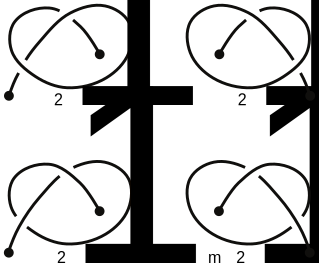
\includegraphics{involutions}
\caption{Knotoid $2_1$ with its symmetric $2_1s$, mirror $2_1m$ and mirror symmetric $2_1ms$.}\label{fig:involutions}
\end{figure}


A table with knotoids on the sphere with up to 5 crossings already exists\cite{bartholomew}. However, here\footnote{when using internal database with \lstinline{--names-db=internal} or with files \lstinline{examples/knotoid_names_planar.txt}, \lstinline{examples/knotoid_names_sphere.txt}, \lstinline{examples/knotoid_names_planar_arrow.txt} or \lstinline{examples/knotoid_names_sphere_arrow.txt}} we use a different table based on a complete classification of all knotoids on the plane with up to 5 crossings and of all knotoids on the sphere with up to 6 crossings (see \cite{goundaroulis2019} for more details).

\subsection{\label{sec:theory:knottedcore}Knotted proteins, slipknots and knotted cores}

It is a long standing belief that folded configurations of proteins should provide an insight on the folding pathways that the backbone follows to reach its native state\cite{Crippen74, Connolly80}. In principle, proteins tend to avoid folding into configurations that involve non-trivial topological features such as knots. At a first glance, it may appear as if nature selects with a bias against the formation of knots. However, their existence\cite{taylor2000} tells us that this may not be the case as knots have been observed to contribute in the stability as well as the function of a protein.

A fingerprint matrix is a triangular matrix where  each entry $(i,j)$ corresponds to a subchain with starting index $i$ and ending index $j$, while it carries also the information of the dominant knotoid or knot type  of its corresponding subchain and it is encoded using a colour scale. Moreover, the whole chain corresponds to the lower left part of the matrix and, therefore, the fingerpring matrix provides a detailed overview of the global as well as the local topology of an open chain.
The knotted core is defined as the shortest subchain obtained by progressively altering the length of the whole chain by 1 point without changing the knot(oid) type in the process. Visually, the knotted core is the  point of the path connected region that includes  the full chain and is closer to the diagonal of the fingerprint matrix. In Figure~\ref{fig:3KZN:fingerprint1000} we see the knotoid fingerprint for the protein 3KZN. Note that this definition of the knotted core corresponds to the "top-down" knotted core discussed by Tubiana and coauthors \cite{tubiana2011}.



In open chains the ending index has to be greater than the starting index which leads to the empty upper part of the matrix and thus to the triangular shape of the fingerprint. On the other hand, in closed chains there is not such a restriction\cite{rawdon,rawdon2}. Thus disk matrices provide an ideal representation of the topology closed chains. In this case we use polar coordinates $(r, \theta)$ to read the matrices, where $r$ corresponds to the length of the subchain and $\theta$ corresponds to the midpoint of the subchain (see Figure~\ref{fig:3KZN:disk}). In analogy to the fingerprint matrix, the knotted core is the  point of the path connected region that includes  the full chain and is closer to the center of the disk matrix.

Apart from knotoids and knots, slipknots also seem to provide valuable information on protein folding\cite{yeates}. Slipknotting appears when a part of the protein backbone forms a knot and then it doubles back so that a non-minimal diagram of the unknot is formed\cite{yeates}. Slipknots can be also generalized to the case of knotoids, where the only difference lies in the fact that the chain may also correspond to a non-minimal non-trivial knotoid. In order to detect slipknots, one has to study all possible subchains of the initial chain. Each subchain is evaluated for the knot or the knotoid type it posseses and the results are summarized in the fingerprint\cite{yeates, sulkowska2012,gound} or disk matrix\cite{rawdon}.
A slipknot can then be visualized as a  region of the matrix that corresponds to a non-trivial knot(oid) and  is disconnected from the region containing the full chain.



\clearpage
